\documentclass[12pt]{article} 
\usepackage{amsmath} 
\usepackage[dvips]{graphicx}
\usepackage{multirow} 
\usepackage{geometry} 
\usepackage{pdflscape}
\usepackage{amsmath}
\usepackage[labelfont=bf]{caption} 
\usepackage{setspace}
\usepackage[running]{lineno} 
% \usepackage[numbers,sort]{natbib}
\usepackage[sort]{natbib} 
\usepackage{array}
\usepackage[table]{xcolor}
\usepackage{xr}
\usepackage{indentfirst}

\newcommand{\methods}{\textit{Materials \& Methods}}
\newcommand{\SI}{\textit{Appendix}~}

\topmargin -1.5cm % 0.0cm 
\oddsidemargin 0.0cm % 0.2cm 
\textwidth 6.5in
\textheight 9.0in % 21cm
\footskip 1.0cm % 1.0cm

\usepackage{authblk}


\title{Species motif participation provides unique information about species risk of extinction}

\author{Alyssa R. Cirtwill$^{1*\dagger}$, Anna \r{A}kesson$^{2*}$, Kate L. Wootton$^{3}$, Anna Ekl\"{o}f$^{2}$} 
\date{
\small$^1$Spatial Foodweb Ecology Group\\
Research Centre for Ecological Change\\
Organismal and Evolutionary Biology Research Programm\\
Faculty of Biological and Environmental Sciences\\
University of Helsinki, Helsinki, Finland\\
\medskip
\small$^2$Department of Theoretical Biology, Chemistry, and Physics\\ 
Link\"{o}ping University, Link\"{o}ping, Sweden\\
\medskip
\small$^3$ School of Biological Sciences\\
University of Canterbury, Christchurch, New Zealand\\
\medskip
* Joint first authors\\
\medskip
$^\dagger$ Corresponding author email: alyssa.cirtwill@gmail.com\\
}

\begin{document} 
\maketitle 
\raggedright

\setlength{\parindent}{15pt} 

\section*{Running headline}
Motif participation describes extinction risk

\clearpage

\section*{Summary}

% Now 282 words. Max 350. 
    1. Loss of species in food webs can set in motion a cascade of additional (secondary)  extinctions.
    2. A species' position in a food web (e.g., its trophic level or number of interactions) is known to affect its ability to persist following disturbance. 
    3. These simple measures, however, offer only a coarse description of how species fit into their community. 
    4. One would therefore expect that more detailed structural measures such as  participation in three-species motifs (meso-scale structures which provide information on a species' direct and indirect interactions) will also be related to probability of persistence.
    5. Disturbances affecting the basal resources have particularly strong effects on the rest of the food web. 
    6. However, how disturbances branch out and affect consumer persistence depends on the structural pattern of species interactions in several steps. 
    7. The magnitude, e.g. proportion of basal resources lost, will likely also affect the outcome.     
    8. Here, we analyse whether a consumer's risk of secondary extinction after removal of basal resources depends on the consumer's motif participation and how this relationship varies with the severity of disturbance.
    9. We show that consumer species which participate more frequently in the direct competition motif and less frequently in the omnivory motif generally have higher probability of persistence following disturbance to basal resources.
    10. However, both the strength of the disturbance and the overall network structure (i.e., connectance) affect the strength and direction of relationships between motif participation and persistence.
    11. Motif participation therefore captures important trends in species persistence and provides a rich description of species' structural roles in their communities, but must be considered in the context of network structure as a whole and of the specific disturbance applied.


\section*{Key-words}
    food web, degree, trophic level, omnivory, competition

\clearpage
\begin{spacing}{1.0}
% \linenumbers

\section*{Introduction} 

    A single extinction can, due to the mutual dependencies among species in a food web,  trigger a cascade of additional (secondary) extinctions. 
    A species' risk of secondary extinction depends on its position within a food web~\citep{Santos2021,dunne2009cascading, Eklof2006}.
    For example, higher trophic levels (long paths to basal resources) and lower in-degree (few prey) increase extinction risk~\citep{Allesina2012,binzer2011susceptibility,Eklof2006}.
    These species are more vulnerable because they are impacted by the loss of any species along a long path from basal resources or because they have few alternative resources to replace lost prey.
    The relationships between these relatively simple measures of a species' position in a food web suggest that more detailed measures, such as a species' participation in \emph{meso-scale motifs} are also related to its persistence~\citep{Cirtwill2022Oikos}.
    
    
    Motifs are unique patterns of interacting species that correspond to different sets of direct and indirect interactions, providing a holistic description of meso-scale network structure~\citep{Stouffer2007,Stouffer2012}.
    Some motifs are over-represented in stable food webs, suggesting that the more frequently species participate in these motifs, the more stable the network will be~\citep{Borrelli2015a}. 
    The vector of frequencies with which a species appears in each motif --its \emph{motif participation}-- describes the species' position in the meso-scale structure of a food web and, like degree and trophic level, is easily calculated once the structure of the network is known.
    Importantly, motif participation incorporates information on the positions of focal species' interaction partners.
    Two species might have the same trophic level and in-degree but quite different motif participation if one species's prey are strict specialists and the others' prey are generalists (Fig.~\ref{fig:concept}).
    Since specialists are usually more vulnerable to extinction than generalists, the predator of specialists will be more likely to lose prey and go extinct itself than will a predator of generalists.
    This extra information on the focal species' interaction partners may thus provide extra insight when predicting extinction risk.
    

    We define motif participation using the well-studied three-species motifs~\citep{Milo2004,Stouffer2007,Stouffer2012}. 
    Four of these motifs --the three-species chain, apparent competition, direct competition, and omnivory-- are especially interesting as they are by far the most common in empirical networks~\citep{Stouffer2007, giling2019plant} and more stable than other motifs (i.e., are more likely to retain all three species in the motif) when modelled in isolation~\citep{Borrelli2015a}.
    These four motifs also have clear ecological interpretations and their dynamics explored using Lotka-Volterra models~\citep{Hsu2015}.
    The three-species chain indicates vertical flows of energy and biomass in a network and captures the possibility of indirect interactions across multiple trophic levels (e.g., between a plant and a predator of the plant's herbivore).
    In general, food chains are more likely to be stable when predator-prey body-mass ratios are smaller~\citep{Jonsson1998}.
    The direct competition motif, where two consumers share the same resource, captures the possibility of indirect interactions between consumers by depletion of the shared resource in competitive exclusion~\citep{Hsu2015}. 
    The apparent competition motif indicates a predator which consumes two resources and, by being somewhat generalist, may be able to persist following the loss or reduction of one prey but can also be affected by indirect effects between the linked prey~\citep{Melian2002}.
    Finally, the omnivory motif, where a predator consumes the same resource as its prey, includes  the potential for a plant to have both direct and indirect effects on the predator. 
    Omnivory is less stable in isolation than the other three motifs~\citep{Borrelli2015a}, though there is a region of stable equilibrium for Lotka-Volterra models of omnivory~\citep{Hsu2015}.
    In whole food webs, frequent omnivory has been proposed to both increase and decrease overall stability in different conditions~\citep{McCann1997,Emmerson2004,Monteiro2016}.
    As most of the above studies either model motifs in isolation or examine overall effects on the whole food web, it remains unclear how a particular species' motif participation will affect its specific extinction risk.

    Previous work using dynamical simulations has shown that motif participation is related to persistence after the loss of a single species in the food web~\citep{Cirtwill2022Oikos}, but the relationship between motif participation and persistence in the face of other disturbances remains unclear.
   As the basal resource community is the foundation upon which all other species depend, and loss of basal resource diversity typically causes declines in both abundance and richness of all types of consumers~\citep{scherber2010bottom,Dobson2009food,Georgiadis2007}.
    Moreover, disturbances to the plant community have been shown to affect both the biomass and diversity of consumers~\citep{chen2019plant,scherber2010bottom,li2020bottom}.
    It is therefore crucial to understand how bottom-up effects from disturbance to basal resources affect the rest of the food web.  
    As well as identifying patterns of motif participation that are associated with ability to persist after a loss of basal resources, we are particularly interested in whether the strength of  disturbance affects relationships between motif participation and persistence.
    For example, participation in one motif might be associated with greater extinction risk after a mild disturbance but be associated with less risk when when more basal resources are lost if the direct and indirect interactions within the motif amplify the effect of small disturbances while providing `back-up' resources when many prey are removed by a strong disturbance.

        
    Here, we analyse whether a consumer's risk of secondary extinction after removal of basal resources depends on the consumer's motif participation and how this relationship varies with the severity of disturbance.
    To provide context for these results, we also consider how a consumer's risk of secondary extinction varies with the overall structure of the network, described by the frequency of motifs, network size, and network connectance.
    Finally, because measures of food-web position are not independent, we identify how species' motif participation varies with overall network structure and with in-degree and trophic level.


\section*{Materials and methods}

    \subsection*{Network construction and describing species roles}

        Simulated networks were generated using the niche model, which recreates the structure of empirical networks well~\citep{Williams2000,Stouffer2007}.
        To capture a range of network architectures similar to those in well-studied empirical networks~\citep{Dunne2002,Dunne2002e}, networks with sizes (S) ranging from 50 to 100 species (in steps of 10) and connectances (C) ranging from 0.02 to 0.18 (in steps of 0.04) were simulated. 
        Biologically unlikely networks (i.e., those with extremely long paths between any consumer and basal resources~\citep{Borrelli2014} were removed and replaced with new simulated networks until 100 suitable networks in each combination of size and connectance were obtained.
        All networks were generated using the function ``nichemodel'' within the Julia~\citep{Bezanson2017julia} package \emph{BioEnergeticFoodWebs}~\citep{bioenergfw,Delmas2017}.     
        For full details and a comparison to empirical networks, see \emph{Appendix S1}.

        
        The motif participation of each consumer species was described in each of these simulated networks before applying any disturbance. 
        A species' motif participation (Fig.~\ref{fig:concept}) is the vector of frequencies with which it appears in each type of motif present in a network~\citep{Stouffer2012}.
        As only four unique three-species motifs can appear in acyclic networks, these are four-dimensional vectors. 
        To focus on the relative frequencies of each motif rather than the total number of motifs, participation vectors were normalized by dividing each count by the total number of motifs the species appears in (such that the vector for each species sums to 1).
        Note, however, that this normalization does not fully control for differences due to degree or connectance~\citep{Cirtwill2022Oikos}. 


        Two simpler measures of a species' position within its community were also calculated.
        In-degree is a species' number of prey.
        Trophic level (shortest trophic level; STL) is the length of the shortest food chain between the focal species and any basal resource~\citep{Williams2004}.
        Both simple role measures were calculated in R~\citep{R} using the same algorithm as~\citet{Eklof2013}.

        
        Finally, network ``motif profiles'' --four-dimensional vectors of the number of each three-species motif in each network~\citep{Stouffer2012}-- were calculated to provide context for species' motif participation..
        Together with network size and connectance, these motif profiles describe the structure of the whole network.
        To separate differences in motif structure from differences in network size or connectance (larger and more-connected networks contain more motifs), motif profiles were normalised by dividing the count of each motif by the total count of all motifs. 
        Motif participation and profiles were calculated using the Python package \emph{pymfinder}~\citep{pymfinder}.

    
    \subsection*{Modelling secondary extinction using Bayesian networks}


        Traditionally, there are two main approaches for studying secondary extinctions (i.e., extinctions of species that were not directly disturbed). 
        First, there are topological models where secondary extinctions only occur once a consumer has lost all of its prey~\citep{dunne2009cascading}. 
        Alternatively, dynamical models explicitly simulate population dynamics using a system of differential equations~\citep{binzer2011susceptibility}. 
        Dynamical models include realistic processes such as indirect interactions but are also highly parameter intensive and require much more computation time than topological models. 
        
        
        Bayesian networks, which are much more computationally efficient and less-parameter-intensive (and therefore less sensative to modelling assumptions) than dynamical models~\citep{Eklof2013} but are more realistic than topological models, offer a middle-ground approach \citep{Eklof2013,Haussler2020}. 
        In this framework, a consumer's probability of extinction depends on the fraction of resources lost ($f = k/n$ for a species with $n$ resources, of which $k$ have gone extinct) and on a baseline probability of extinction ($\pi$) which capturing factors that are not related to the network structure (e.g., disease or stochastic extinction of small populations).
        The efficiency of the Bayesian network framework allows us to simulate a range of disturbance severities rather than single species removals as in many previous studies (e.g.,~\citealp[]{Memmott2004,Staniczenko2010,Cirtwill2022Oikos}).


        One limitation to Bayesian networks is that consumers do not affect the extinction probabilities of their resources (i.e., only bottom-up effects are included).
        Nevertheless, Bayesian networks do capture the vast majority of secondary extinctions obtained from fully-fledged dynamical models including top-down and bottom-up effects~\citep{Eklof2013}, and as such are a good proxy for analysing species persistence following extinctions of primary producers in complex food webs.
        As our focus in this study is on bottom-up effects from disturbance of basal resources, Bayesian networks will capture the secondary extinctions of interest.

        
        Bayesian networks also require the creation of acyclic networks so that a strict bottom-up sequence can be followed. 
        This means that cycles where species A eats species B and vice versa or where A eats B eats C eats A must be broken (see \emph{Appendix S1.3} for details).
        Since cyclic and acyclic versions of a network have the same properties in terms of secondary extinctions and the effects on network robustness are very limited~\citep{Allesina2009functional}, this change will not strongly affect consumers' extinction risk in our simulations.

        
        The removal of cycles also affects which motifs can appear in the network. 
        Any motif which contains a cycle is impossible in an acyclic network.
        This means that only four motifs can appear: apparent competition, direct competition, omnivory, and the three-species chain.
        Fortunately, they are also the motifs that are most common in empirical networks~\citep{Stouffer2007}, have been most studied in isolation (e.g.,~\citealp[]{Bascompte2005,Kondoh2008,Laws2013}), have the clearest ecological interpretations and, because of these three properties, are of greatest interest to us.


        \subsubsection*{Modelling consumers' risk of secondary extinction} 
        
           Response of the consumer to changes in $f$ were modelled using a sigmoid non-linear function ($\alpha > 1, \beta > 1$) which most accurately captures the secondary extinctions produced by dynamical models (\citealp[]{Eklof2013}; \emph{Appendix S2.1}).
            The probability of extinction for each species $i$ can therefore be represented using the cumulative density function of a beta distribution:
    		\begin{equation}
    		P(\lnot i|f) = \pi + (1 - \pi) \frac{B(f;\alpha,\beta)}{B(\alpha,\beta)}.
    				\label{betafunc}
            \end{equation}
    		
            If all resource species of a consumer \textit{C} are present ($f = 0$), the extinction probability is $P(\lnot C|f) = \pi$. 
            Similarly, if all resources are extinct ($f = 1$), $P(\lnot C|f)=1$  and the consumer will go extinct.
            If the fraction $f$ is neither 1 nor 0, the non-linear sigmoid curve will determine the response of the consumer, and $P(\lnot C|f)$ is greater if the fraction of resources lost is high. 
            For basal resources, the abiotic resources they require are assumed to be always available.
            Therefore $f=0$ and, following Equation~\ref{betafunc}, $P(\lnot C|f) = \pi$.
            It is assumed that only the fraction, and not the identity, of the resources lost is important. 
            However, the model can easily be modified to incorporate weighted resource interactions \citep[see][]{Eklof2013}.
    		
    		
            After species $i$'s probability of extinction $P(\lnot i|f)$ is calculated using Equation~\ref{betafunc}, Bernoulli trials are used to determine whether the species goes extinct or not. 
            Species are considered extinct if a random number drawn from a uniform distribution $[0-1]$ is less than $P(\lnot i|f)$.
            Moving up through the food web, the simulated extinctions of prey species are used to calculate the fraction of resources lost $f$ for each consumer and Equation~\ref{betafunc} is updated accordingly. 
            This probabilistic method was repeated 100 000 times per network, with unique random draws.
            For each species, probability of persistence (hereafter `persistence') is defined as the fraction of simulations in which the species persists. 
            While there are methods for solving Bayesian networks exactly \citep{Eklof2013}, for larger networks the numerical evaluation above is highly efficient and produces close to identical results \citep{Haussler2020}.
    		
    	
		
        \subsubsection*{Disturbance scenarios}
        
            In our un-disturbed scenario, all species had an extinction probability of $\pi = 0.1$. 
            To simulate various threats to basal resources, making some species more vulnerable to extinction, probability of extinction for all basal species was increased from $0.10$ to $0.5$, in steps of $0.08$. 
            The highest disturbance level, $\pi = 0.5$, corresponds to basal species having a 50\% risk of going extinct. 
            Consumer species retained $\pi=0.1$ in all cases.


	\subsection*{Statistical analysis} 
        
        \subsubsection*{1) Consumer persistence and motif participation}

            To test whether a consumer's probability of persistence was associated with the frequency of each motif in its participation vector (hereafter simply `participation in motif X') and whether this relationship varied with the strength of disturbance, four general linear models were fit with binomial error distribution (GLMs; one per motif included in the Bayesian networks):
            \begin{equation}
            \Psi_{ink} \approx \rho_{i} + \pi_{k} + \rho_{i}\pi_{k} ,
            % S_{n}C_{n} + N_n,
            \label{propreq}
            \end{equation}
            \noindent where $\Psi_{ink}$ is the persistence of species $i$, belonging to network $n$, during disturbance level $k$, $\rho_{i}$ is the proportion of the role of species $i$ that is made up by the focal motif, and $\pi_k$ is the probability of extinction for a basal resource in disturbance level $k$.
            All predictors were centered and scaled before fitting the models.
            
      
            Initially, general linear mixed-effect models (GLMMs) were fit including random  intercepts for the species richness and connectance of network $n$ and for network identity.
            As these models were singular, each random intercept was removed in turn and the model re-fit until it converged (no random effects remaining).
            All models here and below were fit using the R~\citep{R} functions `glm' from the \emph{stats} package and `glmer' from the package \emph{lmerTest}~\citep{lmerTest}.
            
            
            To test whether these general trends were consistent across networks, the distribution of slopes of simplified regressions fit to a single network and level of disturbance were visually examined.
            These models included only participation in the focal motif ($\rho_{i}$ above) and again used a binomial error distribution.
            To aid in interpretation of these single-network models with respect to network size and connectance, an additional set of GLMs was fit including proportion of motif, strength of disturbance, network size, and connectance across all networks (\emph{Appendix S4.1}).



        \subsubsection*{2) Consumer persistence and other network structure metrics}

            The overall structure of a network could also affect consumers' ability to persist following a disturbance.
            Here, the overall network structure was described using the frequency of each motif in the network's motif profile as well as initial network size and connectance.
            To test whether the frequencies of motifs in the network profile were related to the average persistence of all consumers, a set of four GLMs  (one per motif) were fit with binomial error distribution:
                \begin{equation}
                    \overline{\Psi_{nk}} \approx \Bar{\rho}_{n} + \pi_{k} + \Bar{\rho}_{n}\pi_{k},
                    \label{netpropeq}
                \end{equation}
            \noindent where $\overline{\Psi_{nk}}$ is the mean persistence of consumers in network $n$ at disturbance level $k$, $\Bar{\rho}_{n}$ is the frequency of the focal motif in the network's motif profile, and $\pi_k$ is the level of disturbance (probability of extinction for basal resources).
            As with the GLMs relating each consumer's persistence to its motif participation, GLMMs including random effects of network size and connectance and network identity were initially fit but the random effects were removed in order to obtain non-singular models.


            To identify the relationships between large-scale network structure,  mean persistence within a network, and strength of disturbance, a GLM was fit relating mean persistence to network size, connectance, disturbance, and their interactions.
            To confirm known relationships between persistence and in-degree or trophic level and identify how these relationships might vary with disturbance strength, two GLMs were fit with binomial error distribution relating a consumer's persistence to in-degree or STL, disturbance, and the interaction between them (\emph{Appendix S3.1}, Eq. S2-3).
            When relating persistence to STL, random effects of network size and connectance were initially included but removed due to model singularity as above.
            The model for in-degree was non-singular when including these random effects and so they were retained in this case.



        \subsubsection*{3) Motif participation and other network structure metrics}

            Since a network's motif profile and a species' motif participation reflect the same network as other measures (size, connectance, degree, and trophic level), these measures are not independent. 
            The relationships between frequencies of motifs in the network's motif profile and network size, connectance, and their interaction were described using a set of four GLMs with binomial error distribution (Appendix \emph{S3.2}, eq. S4).
            The relationships between frequencies of motifs in a consumer's motif participation vector and network size, connectance, and their interaction were described using a similar set of four GLMs with binomial error distribution.
            Finally, two additional sets of GLMs (eight total) were fit relating participation in each motif to the consumer's in-degree or trophic level (Appendix \emph{S3.2}, Eq. S5-6).

        
\section*{Results}

    \subsection*{Species persistence and motif participation} 

        A species' probability of persistence (hereafter `persistence') was significantly related to its motif participation (Table S1, \emph{Appendix S5}).
        Across all levels of disturbance, persistence increased with increasing participation in the direct competition motif and decreasing participation in the omnivory motif (Fig.~\ref{fig:prop_lmer_all}).
        The relationships between persistence and participation in the other two motifs varied with the strength of disturbance.
        At low levels of disturbance, persistence increased with increasing participation in the three-species chain motif and decreasing participation in the apparent competition motif.
        These trends were reversed at high levels of disturbance.
    

        Within these overall trends, there was substantial variation between networks (Fig.~\ref{fig:density_prop}).
        Distributions of persistence-motif participation relationships varied strongly with connectance, while network size had a much smaller effect (\emph{Appendix S4.2}).
        The relationship between participation in the omnivory motif and persistence was especially variable.
        Increased participation in the omnivory motif were associated with lower  persistence when connectance was low, regardless of network size or strength of disturbance.
        At moderate connectance, however, increased participation in omnivory was associated with greater persistence when disturbance was weak.
        In the most-connected networks, increased participation in omnivory were associated with greater persistence at all levels of disturbance.

        The relationships between persistence and participation in the other motifs were more consistent over different levels of connectance and network size but tended to be strongest in less-connected networks (Fig.~\ref{fig:density_prop}).
        For the apparent competition and three-species chain motifs, the direction of these relationships depended much more strongly on the strength of disturbance than on connectance.
        For the direct competition motif, persistence increased with increasing participation in the motif across all disturbance levels in networks with low and medium connectance.
        In networks with high connectance, however, the distribution of slopes for this relationship was centered around zero at all levels of disturbance.


    \subsection*{Persistence and other network properties}

       Consumers with higher trophic level (STL) were less likely to persist (Fig.~\ref{fig:lm_CS}, Table S3, \emph{Appendix S6.1}).
        The relationship between in-degree and persistence depended on the strength of disturbance.
        Higher in-degree was associated with greater persistence when basal species had low probability of extinction but lower persistence when basal species were highly likely to go extinct.


        The average persistence of all consumers was lower in networks with higher connectance, did not vary significantly with network size (Table S4, \emph{Appendix S6.1}), and  varied with the frequencies of different motifs in the network's motif profile.
        Specifically, average consumer persistence was higher in networks with higher proportions of the apparent competition motif, lower in networks with higher proportions of the omnivory motif, and not significantly related to the frequencies of the three-species chain or direct competition motifs (Fig.~\ref{fig:lm_CS}, Table S5, \emph{Appendix S6.2}).
        There was no significant interaction between the proportion of any motif in the network motif profile and level of disturbance.


    \subsection*{Motif participation and other network properties}


        A species' motif participation varied with its position in the network and with overall network structure (Fig.~\ref{fig:motifs_vs_TL_and_deg}).
        Species with higher in-degree tended to have higher frequencies of participation in the omnivory motif and lower proportions of the other three motifs.
        Species with higher trophic levels tended to have higher proportions of apparent competition and three-species chains and lower proportions of omnivory and direct competition. 
        
        
        Omnivory motif participation generally increased with increasing connectance and network size, but decreased with increasing network size in the most-connected networks (Fig. S7 and Table S6, \emph{Appendix S7}).
        Participation in the apparent competition and three-species chain motifs decreased strongly with increasing connectance but showed little change with changing network size.
        Direct competition motif participation decreased with increasing connectance in small networks and increased with increasing network size in highly-connected networks, but showed little change with connectance in large networks or with network size in less-connected networks.

        
        The network's motif profile also varied with network connectance.
        Specifically, the proportion of the profile made up by the omnivory motif increased significantly  with increasing connectance while the proportions of the other three motifs decreased (though not significantly).
        No proportions of motifs in the profile were significantly related to network size.


\section*{Discussion}
    
    Here we partially fill the knowledge gap surrounding relationships between a species' position in its food web and its ability to persist following disturbance by testing how the persistence of a consumer in a food web depends on its participation in four different motifs, and how this relationship varies with different levels of disturbance to basal resources. 
    We found that motif participation was related to a consumer's persistence in ways not fully explained by simpler measures of network structure. 
    Species participating more frequently in the direct competition motif and less frequently in the omnivory motif are more likely to persist, while the effects of participating in the apparent competition or three-species chain motifs depend on the strength of disturbance.


    Disturbance strength is often neglected when predicting risk of extinction, but proved important in our results.
    Several of the relationships we demonstrated between probability of persistence and species roles changed direction when moving from weak to strong disturbance.
    These simulation results echo other warnings about `tipping points' where previously beneficial traits can become risky~\citep{Latty2019,Golubski2016,Tylianakis2014}.
    For example, at low levels of disturbance a high degree may be protective since species can compensate if one or a few prey are lost. 
    At high disturbance, however, a high-degree species is likely to be affected by disturbances through many paths and therefore have lower persistence.
    This context-dependence contrasts with the general assumption that species with more resources will be less vulnerable~\citep{Allesina2012,binzer2011susceptibility}, though high-degree species may be less vulnerable than we expect if they are able to switch to alternative prey.
    Our model does not include interaction rewiring, but it is possible that predators with many observed prey may also be more able to attack new prey species after a disturbance than specialists.
    These disturbance effects mean that efforts to define a set of target species for conservation interactions must take the current (and future) level of disturbance the community experiences into account.
    

    The relationship between persistence and participation in the apparent competition motif provides a good example of how motifs provide complementary information to simpler measures of a species' network role.
    Species with higher trophic levels tend to participate more frequently in the apparent competition motif and
    species with higher trophic levels generally have lower persistence~\citep{Eklof2006,Eklof2013}. 
    We would therefore expect high participation in the apparent competition motif to also be associated with lower persistence.
    However, this is only true for low disturbance; at high disturbance the opposite relationship holds.
    This change across disturbance levels may be driven by the negative relationship between apparent competition and in-degree and in-degree's negative relationship with persistence.
    However, it is not obvious when trophic level should be the most important predictor of persistence and when in-degree should be most important.
    Such simpler measures of species' positions in a network could therefore be misleading either because they provide conflicting predictions or because our expectations are only reasonable for specific types or levels of disturbance.


    Participation in the omnivory motif likewise provides information about persistence that is not easily obtained from in-degree and trophic level.
    Although omnivory participation decreased with trophic level (as does persistence) and increased with in-degree (as does persistence, except at high disturbance), we found that greater omnivory participation was usually associated with \emph{lower} persistence-- contrary to what we would expect based on trophic level and in-degree.
    The exception to this pattern is found at high connectance, where increased omnivory participation was more likely to have a positive or neutral relationship with consumer persistence, especially at low disturbance levels (Fig.~\ref{fig:density_prop}).
    This is consistent with other studies showing context-dependent effects of omnivory~\citep{bascompte2005simple, Monteiro2016} and particularly beneficial effects when interaction strengths are weak (as will generally be the case at high connectance)~\citep{Emmerson2004}.
    Although omnivory motifs tend to be less stable in isolation the the other motifs we consider here~\citep{Borrelli2015a}, interactions with other species can stabilise even intrinsically unstable omnivory when embedded in a network~\citep{Kratina2012}.
    As well as leading to weaker average interaction strengths, a higher connectance offers many opportunities for additional interactions that could stabilise unstable omnivory.
    

    There are limitations to the approach presented here.
    Most importantly, the Bayesian network framework operates on a strict bottom-up principle and therefore cannot include top-down effects in the extinction risk calculations~\citep{Eklof2013}. 
    Here our focus was to analyze bottom-up affects following disturbances to the basal resources, in which case the Bayesian network approach captures a majority of the secondary extinctions obtained in a fully-fledged dynamical model with much greater efficiency~\citep{Eklof2013}.
    If top-down effects are important for a particular empirical system, however, our simulations may not be accurate. 
    For example, although a recent study using a dynamical model to relate motif participation to persistence after a disturbance found similar trends for omnivory, participation in the direct competition motif was not universally positive~\citep{Cirtwill2022Oikos}.
    In particular, species which frequently appeared in the prey position of the direct competition motif tended to have shorter persistence times after disturbance in that study - possibly due to top-down effects from the pair of predators involved.
    However, as these two studies applied different types of disturbances, further study would be required to disentangle the effects of top-down and bottom-up effects on species with different motif participation, and how each relates to the type and strength of disturbance.
    Another potentially useful addition to future work would be to include species traits such as body size, which are related to both motif participation~\citep{cirtwill2018feeding} and extinction risk~\citep{Brose2017,Cardillo2005,Purvis2000} in empirical webs.
    
    
    \subsection*{Conclusions}
    
    Many ecologists, including ourselves, have argued that simple measures of species' roles within food webs are important for understanding species' extinction risk~\citep{Santos2021,dunne2009cascading, Eklof2006,binzer2011susceptibility}. 
    However, here we show that relationships between extinction risk and measures of a species' place in its food web are likely more complex, varying with the strength of disturbance and the overall network structure.
    This context-dependence means that even limited changes in network structure or the type of disturbance could change which species are most sensitive to disturbance. 
    As such, caution and increased attention to both network structure and the specifics of disturbance are needed for targeted conservation actions to be most effective. 
    
\section*{Acknowledgements}

    The authors thank Gy\"{o}rgy Barab\'{a}s for excellent discussion of the ideas in this manuscript. A{\AA} is supported by the Swedish Research Council for Sustainable Development Formas (\#2015-01262) granted to AE. ARC is supported by a Finnish Academy postdoctoral research grant (\#332999). ARC, A\r{A}, and AE conceived the study. ARC and KLW simulated networks. A\r{A} and ARC conducted analyses. All authors contributed to writing the manuscript.

% \clearpage    

\bibliographystyle{jae} 
\bibliography{anna_bib_new} 

\clearpage

\section*{Figure legends}
    

        \begin{figure}[hb!]
        \centering
        % 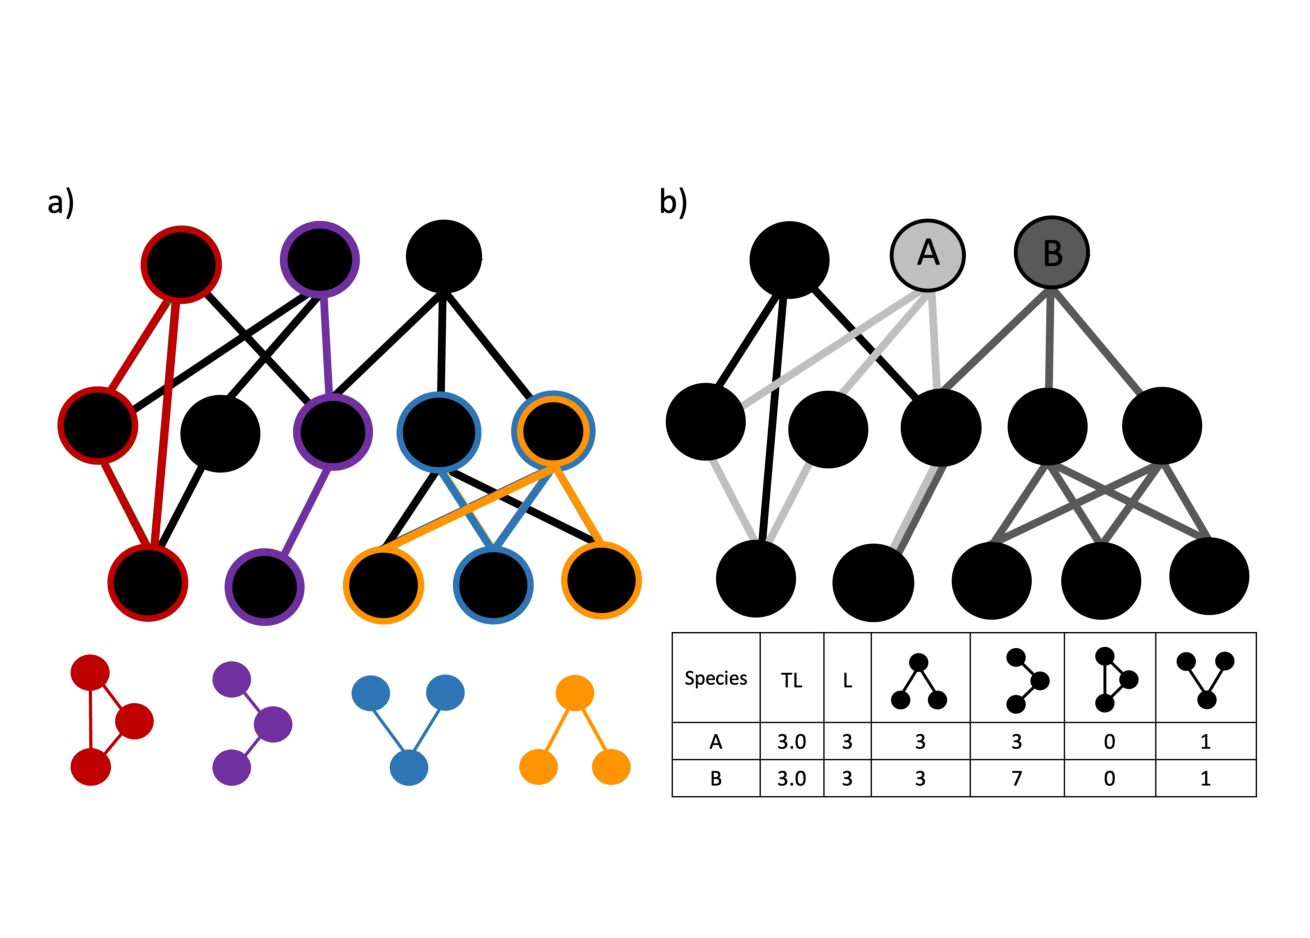
\includegraphics[width=.9\textwidth]{figures/Figure_1.eps}
        \caption{Conceptual figure of a toy food web. \textbf{a)} This food web contains examples of the four motifs: apparent competition (orange), three-species chain (purple), omnivory (red), and direct competition (blue). These motifs capture different ways in which disturbances to basal resources can propagate through the network. For example, a disturbance to the bottom species in a three-species chain will have a direct effect on the middle species but only indirectly affect the top species while a disturbance to the bottom species in an omnivory motif will have a direct effect on the middle species and direct and indirect effects on the top species. 
        Note that the nodes participate in more motifs than the ones highlighted and that a species' motif participation vector is the count of all motifs of each type in which the species appears. \textbf{b)} In the same food web, species with identical degree and trophic level can have different motif participation; here species A (light grey node with links in the same motif colored light grey) participates in only three chains while species B (dark grey node with its direct consumption links colored dark grey) participates in seven (see inserted table for counts of participation in all four motifs; species A has the motif participation vector [3, 3, 0, 1] while species B has the motif participation vector [3, 7, 0, 1]).
        Despite having equal degree and trophic level, species A may be at greater risk of going extinct than species B because of its dependence on specialist prey species. Two-thirds of the prey of species B are generalists and therefore more likely to survive a disturbance to basal resources. By including information about indirect interactions, motif profiles reflect this difference between species A and B while trophic level and degree do not.}
    \label{fig:concept}
    \end{figure}


        \begin{figure}[hb!]
        \centering
        % \includegraphics[width=0.95\textwidth]{figures/persistence_motif_participation.eps}
        \caption{The effect of proportion of the role (x-axis) made up by various motifs (columns) on probability of persistence following disturbance to basal resources (y-axis). The effect of participating in each motif is based on the Equation~\ref{propreq}. The different colored lines indicate the probability of extinction of basal species, from $\pi_{disturbed} = 0.1$ (top, purple; no disturbance) to $\pi_{disturbed} = 0.5$ (bottom, yellow; high disturbance). 95\% confidence intervals for each line are shown in lighter shading. Note that omnivory made up a smaller proportion of species' roles than other motifs; lines are plotted over the observed ranges of motif participation.}
    \label{fig:prop_lmer_all}
    \end{figure}
        
    \begin{figure}[hb!]
    \centering
        % 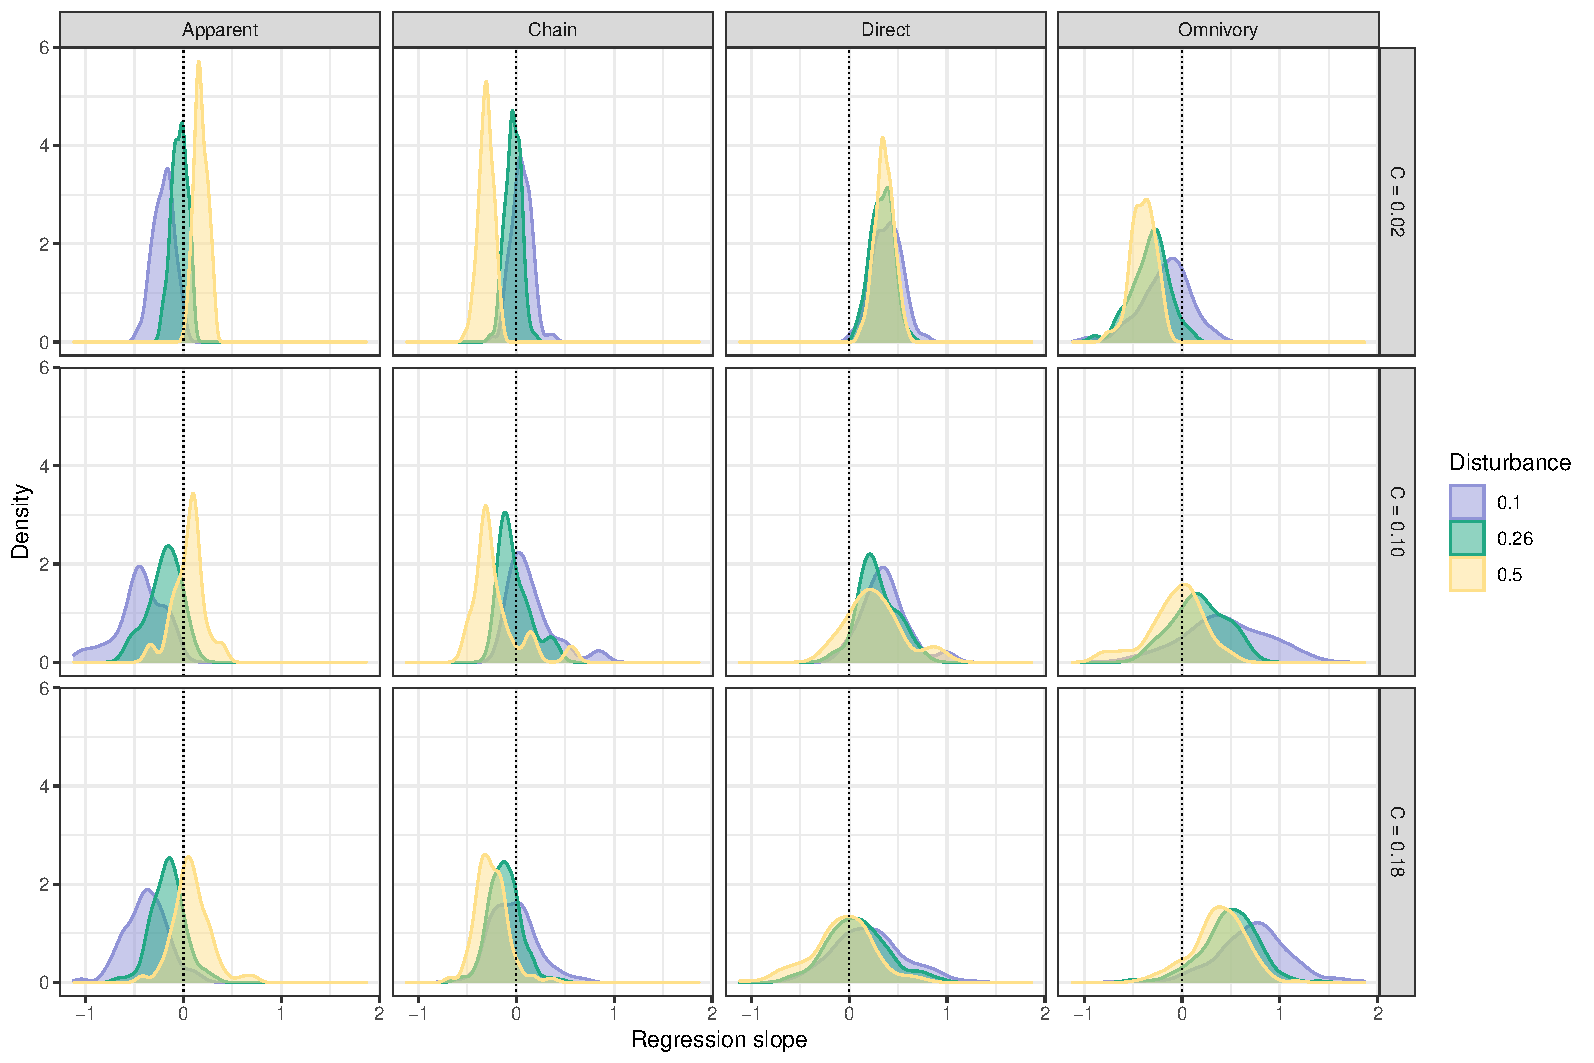
\includegraphics[width=\textwidth]{figures/Fig4.pdf}
        \caption{Here we show the density (y-axis) of slopes (x-axis) of persistence against proportion of different motifs for all simulated webs of all sizes - a visualization of how an increased proportion of each motif (different colored lines) affects persistence of consumer species. Columns show the result for different motifs, rows show results for low, medium, and high connectance, and colour indicates the strength of disturbance to basal resources ($\pi_{disturbed}$; probability of extinction for a basal resource). The dotted, vertical lines indicate zero on the x-axis. A negative slope value reflects a negative relationship between increased participation in a motif and persistence, while a positive slope value reflects a positive relationship - an increased proportion of a specific motif increases persistence.}
        \label{fig:density_prop}
    \end{figure}    


    \begin{figure}[ht!]
        \centering
        % \includegraphics[width=\textwidth]{figures/persistence_vs_SC_lm.eps}
        \caption{The probabilities of persistence for a particular consumer (\textbf{A, B}) and the average probability of persistence across all consumers (\textbf{C-E}) varied with other elements of network structure as well as with motif participation.
        \textbf{A} Persistence of consumers decreased with increasing STL at all levels of disturbance.
        \textbf{B} Persistence of consumers increased with increasing in-degree when the probability of extinction for basal resources was low but decreased with increasing in-degree when the probability of extinction was high.
        \textbf{C,D} Mean persistence of consumers in a network decreased strongly with increasing probability of disturbance to basal resources and decreased slightly, but significantly, with increasing connectance. There was no significant relationship between mean persistence and network size.
        \textbf{E} Mean persistence of consumers decreased with increasing proportions of omnivory in the network's motif profile and increased with increasing proportions of other motifs. Persistence also decreased significantly with increasing probability of basal species extinction but there was no significant interaction; we therefore show trends only for $\pi$=0.1.}
        \label{fig:lm_CS}
    \end{figure}

    \begin{figure}[hb!]
        \centering
        % \includegraphics[width=\textwidth]{figures/roles_vs_TL.eps}
        \caption{Motif participation correlated with in-degree and trophic level, and both of these simpler role measures were also correlated with persistence. \textbf{A)} The proportion of omnivory increased with increasing degree while all other proportions decreased. \textbf{B)} The proportions of omnivory and direct competition decreased with increasing STL while the proportions of apparent competition and three-species chains increased. \textbf{C-D)} The proportion of each motif in consumer's participation vectors varied with connectance, network size, and their interaction (except for apparent competition, where the interaction was not significant). To cover the largest range of slopes, we show relationships over connectance for the smallest networks (\textbf{C}) and over network size for the most-connected networks (\textbf{D}). See also Fig. S6.}
        \label{fig:motifs_vs_TL_and_deg}
    \end{figure}        

\end{spacing}

\end{document}

